\subsection{Well}
In order to build CMOS (Complementary metal–oxide–semiconductor/P and N MOS) on the same substrate an n-well is required for building the complementary P-channel transistor for a n-p-channel logic circuitry as shown above in the example section.
The n-well will serve us as an island of n-doped substrate within the p-doped basis substrate.
The cross section as well as the top view of the targeted geometry are shown below.

\begin{center}
	
\begin{tikzpicture}[node distance = 3cm, auto, thick,scale=0.3, every node/.style={transform shape}]
		% substrate
		\fill[YellowOrange] (0,0) rectangle (20,2);
		\node at (2,0.5) {Si (p-type)};
		% n-well
		\fill[Goldenrod] (1.25,0.75) rectangle (8.25,2);
		\node at (4.75,1) {N-Well};
	\end{tikzpicture}
	
\begin{tikzpicture}[node distance = 3cm, auto, thick,scale=0.3, every node/.style={transform shape}]
		% substrate
		\fill[YellowOrange] (0,0) rectangle (20,12);
		% n-well
		\fill[Goldenrod] (1.25,1.5) rectangle (8.25,7.25);
	\end{tikzpicture}
\end{center}

\subsubsection{Dioxide layer}
In order to selectively inject charge carrying atoms into the crystalline structure a protective dioxide ($SiO_2$) layer needs to be grown on top of a p-type substrate.
\begin{center}
	
\begin{tikzpicture}[node distance = 3cm, auto, thick,scale=0.3, every node/.style={transform shape}]
		% substrate
		\fill[YellowOrange] (0,0) rectangle (20,2);
		\node at (2,0.5) {Si (p-type)};
	\end{tikzpicture}

	
\includegraphics[scale=0.01]{down_arrow.png}

	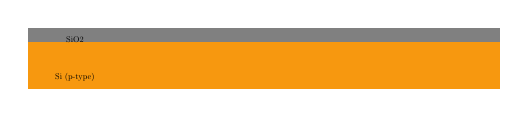
\begin{tikzpicture}[node distance = 3cm, auto, thick,scale=0.3, every node/.style={transform shape}]
		% substrate
		\fill[YellowOrange] (0,0) rectangle (20,2);
		\node at (2,0.5) {Si (p-type)};
		% oxide
		\fill[gray] (0,2) rectangle (20,2.6);
		\node at (2,2.1) {SiO2};
	\end{tikzpicture}
\end{center}
The industrial best practice is a layer of around (500nm$\approx$5000\normalfont\AA) thickness or more.
For this purpose the wafer is being oxidized for at least 90 minutes at 1000\degree C using wet oxidation which results in a dioxide layer at least 500nm($\approx$5000\normalfont\AA) in thickness.

\subsubsection{Patterning}
The resist is being deposited using spin coating and then baked depending on the baking time for the specific resist.
The layout for being exposed onto the resist is being extracted from the "nwell" layer within the GDS2 file.
\begin{center}
	
\begin{tikzpicture}[node distance = 3cm, auto, thick,scale=0.2, every node/.style={transform shape}]
		% substrate
		\fill[YellowOrange] (0,0) rectangle (20,2);
		\node at (2,0.5) {Si (p-type)};
		% oxide
		\fill[gray] (0,2) rectangle (20,2.6);
	\end{tikzpicture}
	
\begin{tikzpicture}[node distance = 3cm, auto, thick,scale=0.2, every node/.style={transform shape}]
		% resist
		\fill[gray] (0,0) rectangle (20,12);
	\end{tikzpicture}

	
\includegraphics[scale=0.01]{down_arrow.png}

	
\begin{tikzpicture}[node distance = 3cm, auto, thick,scale=0.2, every node/.style={transform shape}]
		% substrate
		\fill[YellowOrange] (0,0) rectangle (20,2);
		\node at (2,0.5) {Si (p-type)};
		% oxide
		\fill[gray] (0,2) rectangle (20,2.6);
		% resist
		\fill[orange] (0,2.6) rectangle (1.25,3.2);
		\fill[orange] (8.25,2.6) rectangle (20,3.2);
	\end{tikzpicture}
	
\begin{tikzpicture}[node distance = 3cm, auto, thick,scale=0.2, every node/.style={transform shape}]
		% resist
		\fill[orange] (0,0) rectangle (20,12);
		% substrate
		\fill[gray] (1.25,1.5) rectangle (8.25,7.25);
	\end{tikzpicture}
\end{center}
The thickness of the resist layer and the backing duration will variate depending on the specific equipment for which this process will be implemented with.

\subsubsection{Etching}
\begin{center}
	
\begin{tikzpicture}[node distance = 3cm, auto, thick,scale=0.2, every node/.style={transform shape}]
		% substrate
		\fill[YellowOrange] (0,0) rectangle (20,2);
		\node at (2,0.5) {Si (p-type)};
		% oxide
		\fill[gray] (0,2) rectangle (20,2.6);
		% resist
		\fill[orange] (0,2.6) rectangle (1.25,3.2);
		\fill[orange] (8.25,2.6) rectangle (20,3.2);
	\end{tikzpicture}
	
\begin{tikzpicture}[node distance = 3cm, auto, thick,scale=0.2, every node/.style={transform shape}]
		% resist
		\fill[orange] (0,0) rectangle (20,12);
		% substrate
		\fill[gray] (1.25,1.5) rectangle (8.25,7.25);
	\end{tikzpicture}

	
\includegraphics[scale=0.01]{down_arrow.png}

	
\begin{tikzpicture}[node distance = 3cm, auto, thick,scale=0.2, every node/.style={transform shape}]
		% substrate
		\fill[YellowOrange] (0,0) rectangle (20,2);
		\node at (2,0.5) {Si (p-type)};
		% oxide
		\fill[gray] (0,2) rectangle (1.25,2.6);
		\fill[gray] (8.25,2) rectangle (20,2.6);
		% resist
		\fill[orange] (0,2.6) rectangle (1.25,3.2);
		\fill[orange] (8.25,2.6) rectangle (20,3.2);
	\end{tikzpicture}
	
\begin{tikzpicture}[node distance = 3cm, auto, thick,scale=0.2, every node/.style={transform shape}]
		% resist
		\fill[orange] (0,0) rectangle (20,12);
		% substrate
		\fill[YellowOrange] (1.25,1.5) rectangle (8.25,7.25);
	\end{tikzpicture}
\end{center}

\subsubsection{Cleaning}
\begin{center}
	
\begin{tikzpicture}[node distance = 3cm, auto, thick,scale=0.3, every node/.style={transform shape}]
		% substrate
		\fill[YellowOrange] (0,0) rectangle (20,2);
		\node at (2,0.5) {Si (p-type)};
		% oxide
		\fill[gray] (0,2) rectangle (1.25,2.6);
		\fill[gray] (8.25,2) rectangle (20,2.6);
		% resist
		\fill[orange] (0,2.6) rectangle (1.25,3.2);
		\fill[orange] (8.25,2.6) rectangle (20,3.2);
	\end{tikzpicture}

	
\includegraphics[scale=0.01]{down_arrow.png}

	
\begin{tikzpicture}[node distance = 3cm, auto, thick,scale=0.3, every node/.style={transform shape}]
		% substrate
		\fill[YellowOrange] (0,0) rectangle (20,2);
		\node at (2,0.5) {Si (p-type)};
		% oxide
		\fill[gray] (0,2) rectangle (1.25,2.6);
		\fill[gray] (8.25,2) rectangle (20,2.6);
	\end{tikzpicture}
\end{center}

\subsubsection{Predeposition}
\begin{center}
	\begin{tikzpicture}[node distance = 3cm, auto, thick,scale=0.3, every node/.style={transform shape}]
		% substrate
		\fill[YellowOrange] (0,0) rectangle (20,2);
		\node at (2,0.5) {Si (p-type)};
		% oxide
		\fill[gray] (0,2) rectangle (1.25,2.6);
		\fill[gray] (8.25,2) rectangle (20,2.6);

		\newcounter{ct}
		\forloop{ct}{0}{\value{ct} < 21}
		{
			\draw [->] (\value{ct},4) -- (\value{ct},3);
			\node at (\value{ct},4.2) {P$^{31}$};
		}
	\end{tikzpicture}

	
\includegraphics[scale=0.01]{down_arrow.png}

	
\begin{tikzpicture}[node distance = 3cm, auto, thick,scale=0.3, every node/.style={transform shape}]
		% substrate
		\fill[YellowOrange] (0,0) rectangle (20,2);
		\node at (2,0.5) {Si (p-type)};
		% phosphorus
		\fill[Goldenrod] (1.25,1.8) rectangle (8.25,2);
		\node at (4.75,1.9) {n+};
		% oxide
		\fill[gray] (0,2) rectangle (1.25,2.6);
		\fill[gray] (8.25,2) rectangle (20,2.6);

		\fill[Goldenrod] (0,2.5) rectangle (1.25,2.6);
		\fill[Goldenrod] (8.25,2.5) rectangle (20,2.6);
	\end{tikzpicture}
\end{center}
The n-well is implanted with a Phosphorus ($P^{31}$) dose of $2.5\times10^{12}cm^{-2}$ at an energy of 100 KeV.
The n-well is then annealed.

\subsubsection{Sacrificial oxide}
\begin{center}
	
\begin{tikzpicture}[node distance = 3cm, auto, thick,scale=0.3, every node/.style={transform shape}]
		% substrate
		\fill[YellowOrange] (0,0) rectangle (20,2);
		\node at (2,0.5) {Si (p-type)};
		% phosphorus
		\fill[Goldenrod] (1.25,1.8) rectangle (8.25,2);
		\node at (4.75,1.9) {n+};
		% oxide
		\fill[gray] (0,2) rectangle (1.25,2.6);
		\fill[gray] (8.25,2) rectangle (20,2.6);

		\fill[Goldenrod] (0,2.5) rectangle (1.25,2.6);
		\fill[Goldenrod] (8.25,2.5) rectangle (20,2.6);
	\end{tikzpicture}

	
\includegraphics[scale=0.01]{down_arrow.png}

	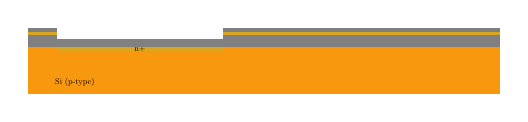
\begin{tikzpicture}[node distance = 3cm, auto, thick,scale=0.3, every node/.style={transform shape}]
		% substrate
		\fill[YellowOrange] (0,0) rectangle (20,2);
		\node at (2,0.5) {Si (p-type)};
		% phosphorus
		\fill[Goldenrod] (1.25,1.8) rectangle (8.25,2.0);
		\node at (4.75,1.9) {n+};
		% oxide
		\fill[gray] (0,2) rectangle (1.25,2.8);
		\fill[gray] (1.25,2) rectangle (8.25,2.3);
		\fill[gray] (8.25,2) rectangle (20,2.8);
		
		\fill[Goldenrod] (0,2.5) rectangle (1.25,2.6);
		\fill[Goldenrod] (8.25,2.5) rectangle (20,2.6);
	\end{tikzpicture}
\end{center}

The wafer is being oxidized for 32 minutes at 1000\degree C in order to achieve a cover silicon layer of 250nm thickness ($\approx$2500\normalfont\AA).

\subsubsection{Infusion}
In order to drive the carrier atoms deeper into the crystalline structure the wafer needs to be driven in after predeposition.
\begin{center}
	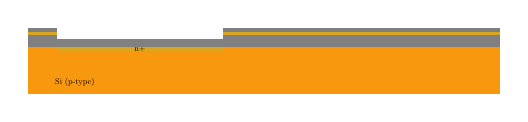
\begin{tikzpicture}[node distance = 3cm, auto, thick,scale=0.3, every node/.style={transform shape}]
		% substrate
		\fill[YellowOrange] (0,0) rectangle (20,2);
		\node at (2,0.5) {Si (p-type)};
		% phosphorus
		\fill[Goldenrod] (1.25,1.8) rectangle (8.25,2.0);
		\node at (4.75,1.9) {n+};
		% oxide
		\fill[gray] (0,2) rectangle (1.25,2.8);
		\fill[gray] (1.25,2) rectangle (8.25,2.3);
		\fill[gray] (8.25,2) rectangle (20,2.8);
		
		\fill[Goldenrod] (0,2.5) rectangle (1.25,2.6);
		\fill[Goldenrod] (8.25,2.5) rectangle (20,2.6);
	\end{tikzpicture}

	
\includegraphics[scale=0.01]{down_arrow.png}

	
\begin{tikzpicture}[node distance = 3cm, auto, thick,scale=0.3, every node/.style={transform shape}]
		% substrate
		\fill[YellowOrange] (0,0) rectangle (20,2);
		\node at (2,0.5) {Si (p-type)};
		% n-well
		\fill[Goldenrod] (1.25,0.75) rectangle (8.25,2);
		\node at (4.75,1) {N-Well};
		% oxide
		\fill[gray] (0,2) rectangle (1.25,2.8);
		\fill[gray] (1.25,2) rectangle (8.25,2.3);
		\fill[gray] (8.25,2) rectangle (20,2.8);
		
		\fill[Goldenrod] (0,2.5) rectangle (0.25,2.6);
		\fill[Goldenrod] (8.25,2.5) rectangle (20,2.6);
	\end{tikzpicture}
\end{center}
In this step the wafer is  driven-in for 960 minutes at 1150\degree C in an inert ambient.

\subsubsection{Oxide removal}
We want an oxide free wafer with the n-well accessible for the further process steps.
\begin{center}
	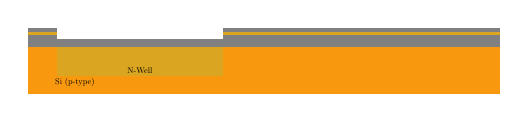
\begin{tikzpicture}[node distance = 3cm, auto, thick,scale=0.3, every node/.style={transform shape}]
		% substrate
		\fill[YellowOrange] (0,0) rectangle (20,2);
		\node at (2,0.5) {Si (p-type)};
		% n-well
		\fill[Goldenrod] (1.25,0.75) rectangle (8.25,2);
		\node at (4.75,1) {N-Well};
		% oxide
		\fill[gray] (0,2) rectangle (1.25,2.8);
		\fill[gray] (1.25,2) rectangle (8.25,2.3);
		\fill[gray] (8.25,2) rectangle (20,2.8);
		
		\fill[Goldenrod] (0,2.5) rectangle (1.25,2.6);
		\fill[Goldenrod] (8.25,2.5) rectangle (20,2.6);
	\end{tikzpicture}
	
	
\includegraphics[scale=0.01]{down_arrow.png}

	
\begin{tikzpicture}[node distance = 3cm, auto, thick,scale=0.3, every node/.style={transform shape}]
		% substrate
		\fill[YellowOrange] (0,0) rectangle (20,2);
		\node at (2,0.5) {Si (p-type)};
		% n-well
		\fill[Goldenrod] (1.25,0.75) rectangle (8.25,2);
		\node at (4.75,1) {N-Well};
	\end{tikzpicture}
\end{center}
We use hydrofluoric acid, because it doesn't etch silicon at all but is very aggressive towards $SiO_2$

For hydrofluoric acid in combination with $SiO_2$ the following reaction formula can be used
\begin{equation}
4 H F_{(aq]} + SiO_{2(s]} \rightarrow SiF_{4(g]} \uparrow + 2 H_{2} O_{(l]}
\end{equation}
while with non oxidized silicon there is no reaction.